\section{Beispiele für Zero-Knowledge-Beweise}

\subsection{Graphenisomorphismus}
\begin{definition}[Graphenisomorphismus]
Gegeben seien zwei Graphen \( G_0 = \left( V_0, E_0 \right) \) und \( G_1 = \left( V_1, E_1 \right) \). Beide Graphen sind genau dann isomorph zueinander, wenn man einen Graphen durch Umbenennung der Knoten in den anderen umwandeln kann. Die Sprache der isomorphen Graphen ist somit

\[ L_{isomorph} = \left\lbrace \left( G_0, G_1 \right) \mid \exists \phi \in S_{\left| V_0 \right|}: G_0 = \phi \circ G_1 \right\rbrace \]

wobei \( S_n \) die \textnormal{Symmetrische Gruppe}, also die Menge aller Permutationen über \( n \) Elementen, bezeichne.
\end{definition}
 
\vspace{1em}
\begin{minipage}{\linewidth}
	\centering
	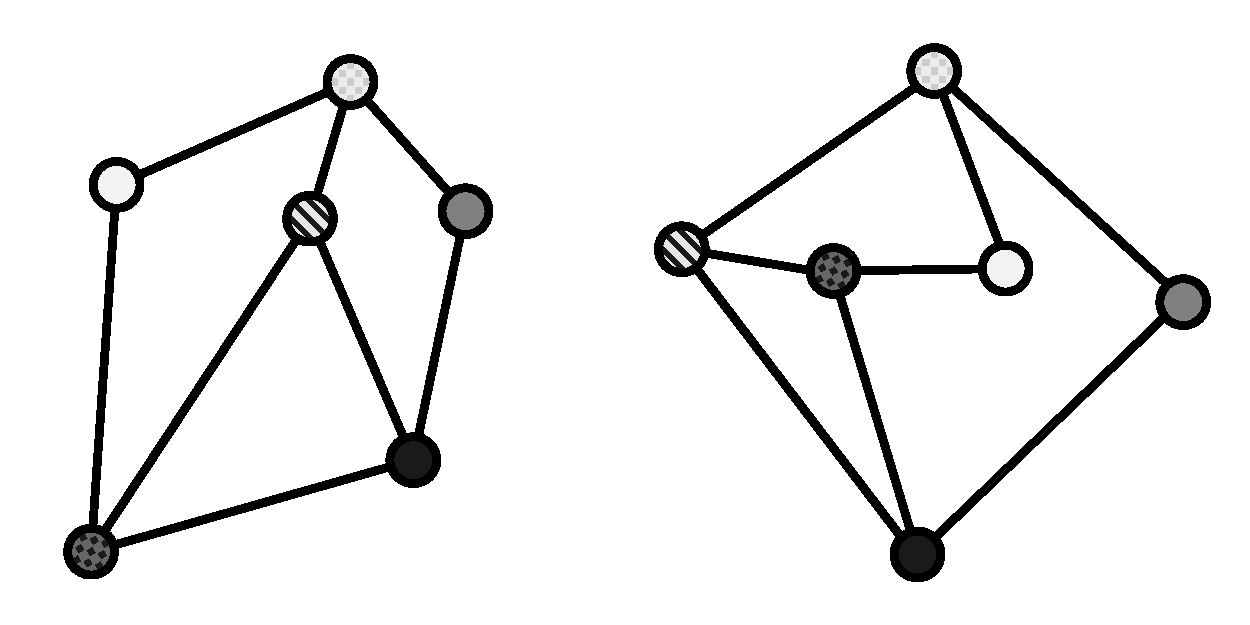
\includegraphics[width=0.7\linewidth]{img/isomorphism-example.pdf}
	\captionof{figure}[Zwei zueinander isomorphe Graphen]{Zwei zueinander isomorphe Graphen. Der Isomorphismus ist durch die gleiche Einfärbung der Knoten visualisiert.}
	\label{fig:isomorphism}
\end{minipage}

\subsubsection{Zero-Knowledge-Beweisprotokoll}

\begin{protocol}[Graphenisomorphismus]
\label{protocol:isomorphism}
Gemeinsame Eingabe: \( G_0 = \left( V_0, E_0 \right) \) und \( G_1 = \left( V_1, E_1 \right) \).\\
Geheime Eingabe an den Beweiser: Isomorphismus zwischen beiden Graphen \( \phi \) mit \( G_0 = \phi \circ G_1 \).
\begin{itemize}
\item[(Beweiser, Schritt 1)] Ziehe zufällige Permutation \( \pi_0 \in S_{\left| V_0 \right| } \) und sende \( G' = \pi_0 \circ G_0 \) an den Verifizierer
\item[(Verifizierer, Schritt 1)] Ziehe zufälliges Bit \( \alpha \in \left\lbrace 0, 1 \right\rbrace \) und sende es an den Beweiser. Implizit bedeutet dies, dass bei \( 0 \) die Permutation \( \pi_0 \) gezeigt werden soll, bei \( 1 \) die Permutation \( \pi_1 \) mit \( G' = \pi_1 \circ G_1 \)
\item[(Beweiser, Schritt 2)] Falls \( \alpha = 1 \), sende \( \pi_1 = \pi_0 \circ \phi \) an den Verifizierer, sonst \( \pi_0 \)
\item[(Verifizierer, Schritt 2)] Akzeptiere, falls \( G' = \pi_\alpha \circ G_\alpha \), sonst verwerfe\footnote{aus \cite[Protocol 2]{np}}
\end{itemize}
\end{protocol}

\subsubsection{Zero-Knowledge-Eigenschaft}

\begin{theorem}
Bei Protokoll \ref{protocol:isomorphism} handelt es sich um ein interaktives Beweissystem.
\end{theorem}

\begin{proof}
Vollständigkeit: Falls \( G_0 \) und \( G_1 \) tatsächlich isomorph sind, kennt \( P \) nach Voraussetzung den Isomporphismus \( \phi \) und kann somit immer sowohl das zufällig gezogene \( \pi_0 \), als auch \( \pi_1 = \pi_0 \circ \phi \) zurückgeben. \\
Korrektheit: Falls \( G_0 \) und \( G_1 \) nicht isomorph zueinander sind, kann \( G' \) nicht isomporph zu beiden Graphen sein - und somit wird \( P \) mit einer Wahrscheinlichkeit \( \geq \frac{1}{2} \) daran scheitern, einen Isomorphismus von \( G_\alpha \) zu \( G' \) anzugeben.
\end{proof}

Höhere Sicherheiten für den Verifizierer als \( \frac{1}{2} \) können dabei durch eine Wiederholung des Beweises (mit einer neuen Permutation) erzielt werden. Nach zehn Beweisen ist man somit beispielsweise bei einer Wahrscheinlichkeit von \( 99,8 \% \).

Dabei sollte nicht zweimal die gleiche Permutation \( \pi_0 \) verwendet werden, da sonst, falls sich der Verifizierer einmal für \( \alpha = 0 \) und einmal für \( \alpha = 1 \) entscheidet, \( \phi \) einfach durch \( \phi = \pi_0^{-1} \circ \pi_1 \) berechnet werden kann.

% TODO: Abstand einfügen
\vspace{0.2cm}

\begin{theorem}
Protokoll \ref{protocol:isomorphism} ist Zero Knowledge.
\end{theorem}

% TODO: Erklärung, warum V* und nicht mit normalen V 

\begin{proof}
\label{proof:zeroisomorphism}
Sei \( V^{\ast} \) eine beliebige, aber feste im Erwartungswert polynomielle ITM. Die Zero-Knowledge-Eigenschaft des Protokolls kann hier konstruktiv bewiesen werden, also durch die Angabe einer im Erwartungswert polynomiellen Maschine \( M_{V^{\ast}} \), die eine rechnerisch ununterscheidbare Verteilung zu einer Kommunikation mit dem Beweiser \( P \) generiert.

Dabei wird \( V^{\ast} \) von einer im Erwartungswert polynomiellen Turing-Maschine \( M_{V^{\ast}} \) simuliert, wobei dieser die Bandinhalte von 
\( M_{V^{\ast}} \) vorgegeben werden.
Das öffentliche Eingabeband von \( V^{\ast} \) ist damit immer mit \( \left( G_0, G_1 \right) \) beschrieben und das geheime Eingabeband bleibt leer. Das Zufallsband von \( V^{\ast} \) wird mit im Voraus von \( M_{V^{\ast}} \) gezogenen Zufallsbits befüllt, die über die gesamte Simulation gleich blieben. Dadurch wird erzielt, dass das Verhalten von \( V^{\ast} \) bei einer erneuten Simulation nur noch von den Inhalten des nur-lesbaren Kommunikationsbandes abhängt, also deterministisch wird.

Um Zero-Knowledge auch bei mehrfacher Ausführung des Protokolls zu beweisen, werden hier mehrere einzelne Ausführungen nacheinander betrachtet. Die Eingaben und Ausgaben von \( V^{\ast} \) über die Kommunikationsbänder werden dabei in einem Kommunikationsprotokoll festgehalten.

Eine einzelne Simulation einer Durchführung des Protokolls beginnt damit, dass \( M_{V^{\ast}} \) ein zufälliges \( \beta \in \left\lbrace 0, 1 \right\rbrace \) und eine zufällige Permutation in \( \psi \in S_{ \left| V_\beta \right| } \) zieht und anschließend damit \( G' = \psi \circ G_\beta \) berechnet. Damit \glqq{}setzt\grqq{} \( M_{V^{\ast}} \) darauf, dass sich \( V^{\ast} \) für \( \beta \) entscheiden wird. Danach wird \( V^{\ast} \) mit allen bisherigen erfolgreichen Durchführungen des Protokolls und zusätzlich dem Beginn des aktuellen (also das Zusenden von \( G' \)) ausgeführt. Falls das von \( V^{\ast} \) gezogene \( \alpha = \beta \) ist, war dieser Beweisschritt erfolgreich und wird dem Kommunikationsprotokoll angehängt, sonst wird die gesamte einzelne Durchführung des Protokolls verworfen und wiederholt. Wenn die gewünschte Anzahl an Einzeldurchführungen erreicht wurde, werden diese zurückgegeben.

Hier lässt sich zeigen, dass die Verteilungen sogar statistisch Zero Knowledge sind, woraus das schwächere rechnerische Zero Knowledge aus Definition \ref{definition:zeroknowledge} folgt.\footnote{Folgerung aus \cite[Seite 193]{identity}. Ein präziserer Beweis, der diesen Beweis zu Ende führt und noch auf einige weitere Details eingeht ist unter \cite[Theorem 2]{np} zu finden.}
\end{proof}

\subsection{Färbung eines Graphen mit drei Farben}
Ein weiteres Entscheidungsproblem mit einem Zero-Knowledge-Beweis ist die Färbung eines Graphen mit drei Farben:

% TODO: Abstand einfügen
\vspace{0.2cm}

\begin{definition}[G3C]
Gegeben sei ein Graph \( G = \left( V, E \right) \). Ein Graph gehört genau dann zu der Sprache der mit nur drei Farben einfärbbaren Graphen \( L_{G3C} \), wenn jedem Knoten eine von drei verschiedenen Farben (in der Definition die Zahlen \( \left\lbrace 1, 2, 3\right\rbrace \)) so zugewiesen werden kann, dass keine Kante zwei Knoten derselben Farbe verbindet.

\[ 
L_{G3C} = \left\lbrace G = \left( V, E \right) \mid \exists \phi: V \rightarrow \left\lbrace 1, 2, 3\right\rbrace: \forall \left( u, v \right) \in E: \phi \left( u \right) \neq \phi \left( v \right) \right\rbrace	
\]
\end{definition}

\vspace{1em}
\begin{minipage}{\linewidth}
	\centering
	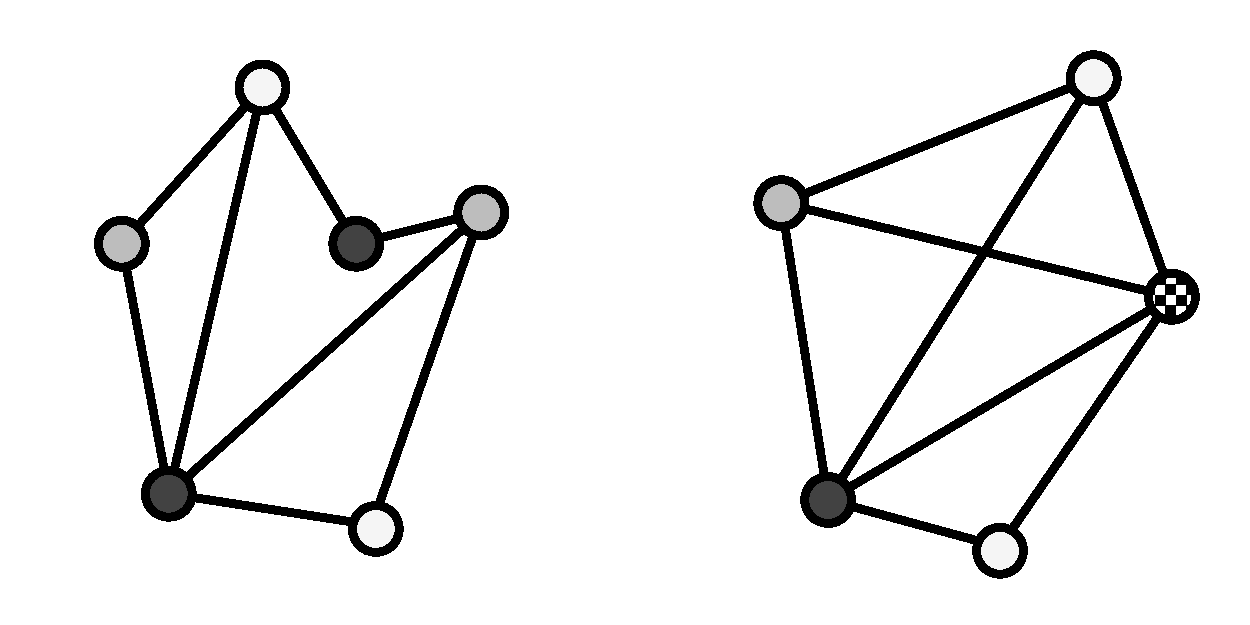
\includegraphics[width=0.7\linewidth]{img/3colorgraphs-example.pdf}
	\captionof{figure}[Beispiel für einen mit drei Farben einfärbbaren (links) und einen nicht mit drei Farben einfärbbaren Graphen (rechts).]{Beispiel für einen mit drei Farben einfärbbaren (links) und einen nicht mit drei Farben einfärbbaren Graphen (rechts).}
	\label{fig:3coloringexample}
\end{minipage}

% TODO: Abstand einfügen
\vspace{0.2cm}

Interessant ist hierbei, dass im Gegensatz zu dem Graphenisomorphismus eine Reduktion von SAT auf die Färbung eines Graphen mit drei verschiedenen Farben exisitert und das Problem damit NP-vollständig ist.\footnote{siehe \cite[Seite 14]{np}} Welche Bedeutung dieser Zero-Knowledge-Beweis somit auf alle Probleme in NP hat, wird nach dem Beweisprotokoll dann in Abschnitt \ref{section:npconsequences} beschrieben. 

\subsubsection{Zero-Knowledge-Beweisprotokoll}
Für diesen Zero-Knowledge-Beweis wird eine sogenannte Einwegfunktion benötigt, mithilfe derer sich der Verifizierer sicher sein kann, dass sich der Beweiser auf einen bestimmten Wert für jeden Knoten festgelegt hat, jedoch nicht auf diese Werte kommen kann. Formal definiert sieht eine solche Funktion wie folgt aus:

\begin{definition}[Einwegfunktion]
Eine Funktion \( f: \left\lbrace 1, 2, 3\right\rbrace \times \left\lbrace 0, 1\right\rbrace ^{\ast} \rightarrow \left\lbrace 0, 1\right\rbrace ^{\ast} \) wird Einwegfunktion genannt, falls folgende Eigenschaften gegeben sind:\footnote{vgl. \cite[Definition 6]{np} und \cite[Definition 2]{20yearszeroknowledge}}

\begin{itemize}
\item[Effiziente Berechenbarkeit:] Die Funktion ist für jede Eingabe in polynomieller Zeit berechenbar.
\item[Kollisionsfreiheit:] \( \forall x, y \in \left\lbrace 1, 2, 3\right\rbrace, x \neq y, r, s \in  \left\lbrace 0, 1\right\rbrace ^{\ast}, r \neq s: f \left( x, r \right) \neq f \left( y, s \right) \)
\item[Sicherheit:] Sei die Zufallsvariable \( f_n \left( x \right) \) definiert als \( f_n \left( x \right) = f \left( x, r_n \right) \) mit jeweils zu\-fäl\-li\-gem \( r_n \in \left\lbrace 0, 1\right\rbrace ^{ n } \) als probabilistische Verschlüsselungsfunktion.
Die Verteilungsfamilien \( \left\lbrace f_n \left( x\right) \right\rbrace_n \) und \( \left\lbrace f_n \left( y\right) \right\rbrace_n \) müssen für alle \( x, y \in \left\lbrace 1, 2, 3\right\rbrace, x \neq y \) rechnerisch ununterscheidbar sein.
\end{itemize}
\end{definition}

Man kann eine Einwegfunktion auch als verschließbare Box ansehen, die vom Beweiser verschlossen an den Verifizierer überreicht wird, der den Inhalt erst dann überprüfen kann, wenn der Beweiser ihm zusätzlich den Schlüssel aushändigt. Der Beweiser kann jedoch, sobald die Box übergeben worden ist, nichts mehr an deren Inhalt ändern.

\begin{protocol}[Kolorierbarkeit mit drei Farben]
\label{protocol:3color}
Gemeinsame Eingabe: \( G = \left( V_G, E_G \right) \).\footnote{aus \cite[Protocol 4]{np}}
Geheime Eingabe an den Beweiser: Korrekte Einfärbung von \( G \): \( \phi : V \rightarrow \left\lbrace 1, 2, 3\right\rbrace \)
\begin{itemize}
\item[(Beweiser, Schritt 1)] Ziehe eine zufällige Permutation \( \pi \) aus \( S_3 \), berechne für jedes \( v \in V_G \) mit einem jeweils eigenen, zufälligen \( r_v \in \left\lbrace 0, 1\right\rbrace ^n \) den Wert \( F_v = f \left( \pi \left( \phi \left( v \right) \right), r_v \right) \) und sende diese
\item[(Verifizierer, Schritt 1)] Ziehe eine zufällige Kante \( \left( u, v \right) \in E \) und sende diese
\item[(Beweiser, Schritt 2)] Falls \( \left( u, v \right) \in E \), schicke dem Verifizierer \( \left( \pi \left( \phi \left( v \right) \right), r_v \right) \) und \( \left( \pi \left( \phi \left( u \right) \right), r_u \right) \)
\item[(Verifizierer, Schritt 2)] Akzeptiere, falls \( F_v \) und \( F_u \) korrekt berechnet worden waren und den beiden verbundenen Knoten unterschiedliche Farben (bzw. hier Zahlen) zugewiesen worden waren, sonst verwerfe
\end{itemize}
\end{protocol}

Der Trick bei diesem Beweis ist, dass dadurch, dass jedes Mal die Farben durch die Permutation \( \pi \) umbenannt werden, der Verifizierer zwar sieht, dass unterschiedliche Farben an zwei benachbarten Knoten verwendet werden, jedoch nicht mehr erfährt, da die Farben zufällig sind.

\vspace{1em}
\begin{minipage}{\linewidth}
	\centering
	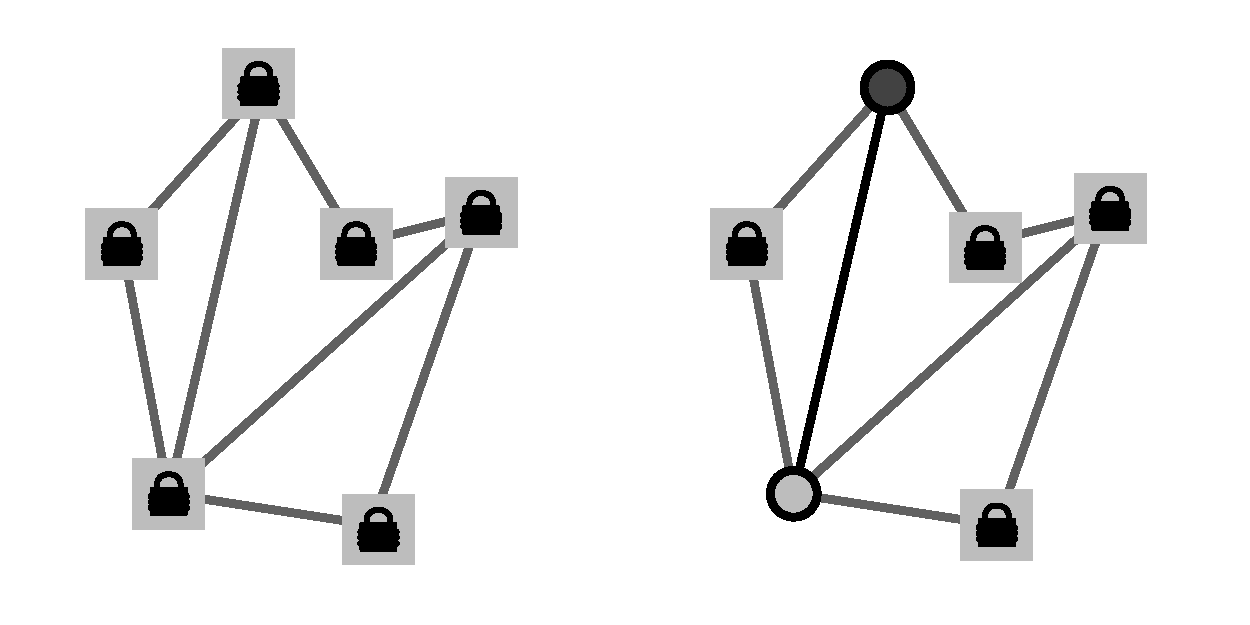
\includegraphics[width=0.7\linewidth]{img/3colorgraphs-proof.pdf}
	\captionof{figure}[Graphische Visualisierung des Beweisprotokolls \ref{protocol:3color}]{Graphische Visualisierung des Beweisprotokolls \ref{protocol:3color}. Links ist zu sehen, was der Beweiser in Schritt 1 sendet, rechts die aufgedeckte Kante aus Schritt 2.}
	\label{fig:3coloringproof}
\end{minipage}

\subsubsection{Zero-Knowledge-Eigenschaften des Beweisprotokolls}

\begin{theorem}
Bei Protokoll \ref{protocol:3color} handelt es sich um ein interaktives Beweissystem.
\end{theorem}

\begin{proof}
Vollständigkeit: Falls \( G \) mit drei Farben einfärbbar ist, kennt \( P \) nach Voraussetzung diese Einfärbung \( \phi \) - und somit kann auch keine Kante entdeckt werden, deren Knoten dieselbe Farbe zugewiesen wurde.\\
Korrektheit: Falls der Graph nicht mit drei Farben korrekt einfärbbar ist, muss es in dem verschlüsselt gesendeten Graphen mindestens eine Kante geben, deren Knoten diesselbe Farbe besitzen. Die Wahrscheinlichkeit dafür, dass diese aufgedeckt wird, beträgt \( \frac{1}{\left| E_G \right|} \). Wie auch im oberen Beweis kann diese Wahrscheinlichkeit durch Mehrfachausführung des Protokolls erhöht werden.
\end{proof}

\begin{theorem}
Bei Protokoll \ref{protocol:3color} ist Zero Knowledge, falls \( f \) eine Einwegfunktion ist.
\end{theorem}

Im Allgemeinen verläuft der Beweis hierzu ähnlich wie bei Satz \ref{proof:zeroisomorphism} - es wird wieder der beliebige Verifizierer \( V^{\ast} \) durch das gleichbleibende Zufallsband deterministisch gemacht und anschließend werdem diesem zufällige Farben für die Knoten verschlüsselt gesendet. Diesmal kann jedoch nur rechnerisches Zero Knowledge (aus Definition \ref{definition:zeroknowledge}) gezeigt werden. Eine Schwierigkeit im Beweis ist, dass der möglicherweise unehrliche Verifizierer seine Entscheidungen auf den verschlüsselten Farben \( \left\lbrace F_v \right\rbrace_{v \in V_G} \) basiert.\footnote{Der vollständige Beweis kann in \cite[Proposition 4]{np} nachgelesen werden.}

\subsection{Folge für alle NP-Probleme}
\label{section:npconsequences}
Da nach \cite{karp} G3C NP-vollständig sind, kann man nun mithilfe der bereits bekannten Reduktionen Zero-Knowledge-Beweise für alle Probleme in NP wie folgt herleiten:

% TODO: Abstand
\vspace{0.2cm}

\begin{theorem}
Falls eine Einwegfunktion exisitiert, besitzt jede Sprache in NP ein interaktives Zero-Knowledge-Beweissystem.
\end{theorem}

\begin{proof}
Sei \( L \) eine beliebige Sprache in \( NP \) und \( g \) eine invertierbare, in polynomieller Zeit ausführbare Reduktion von \( L \) auf SAT. Die ist von jeder Sprache in NP zu (3)SAT durch den Satz von Cook\footnote{siehe \cite{cook}} und mithilfe der Karp-Reduktion\footnote{siehe \cite{karp} als Chromatic Number} weiter zu G3C gegeben. \( g \left( x \right) \) ist somit ein mit drei Farben kolorierbarer Graph.

Bei einer gemeinsamen Eingabe von \( \omega \in L \) berechnen sowohl \( P \) als auch \( V \) den mit drei Farben einfärbaren Graphen \( g \left( \omega \right) \) (und im Falle von \( P\) dessen korrekte Einfärbung)  und führen anschließend den in Protokoll \ref{protocol:3color} gegebenen Beweis aus. Falls dieser erfolgreich ist, akzeptiert \( V \).\footnote{Ein präziserer Beweis ist in \cite[Theorem 5+6]{np} oder \cite[Seite 14]{20yearszeroknowledge} zu finden.}
\end{proof}

\pagebreak